\section{Vehicle description}

\subsection{The vehicle in general}

The vehicle used in this project 

A platform of the same size of the vehicle  is mounted on the vehicle, to support the PCB, the battery, and the sensors used to control the path of the vehicle.\\
\todo{have to put the dimensions and weight of the vehicle}
The drive train is described on \figref{vehicleDescriptionDriveTrain}.

\begin{figure}[H]
	\centering
	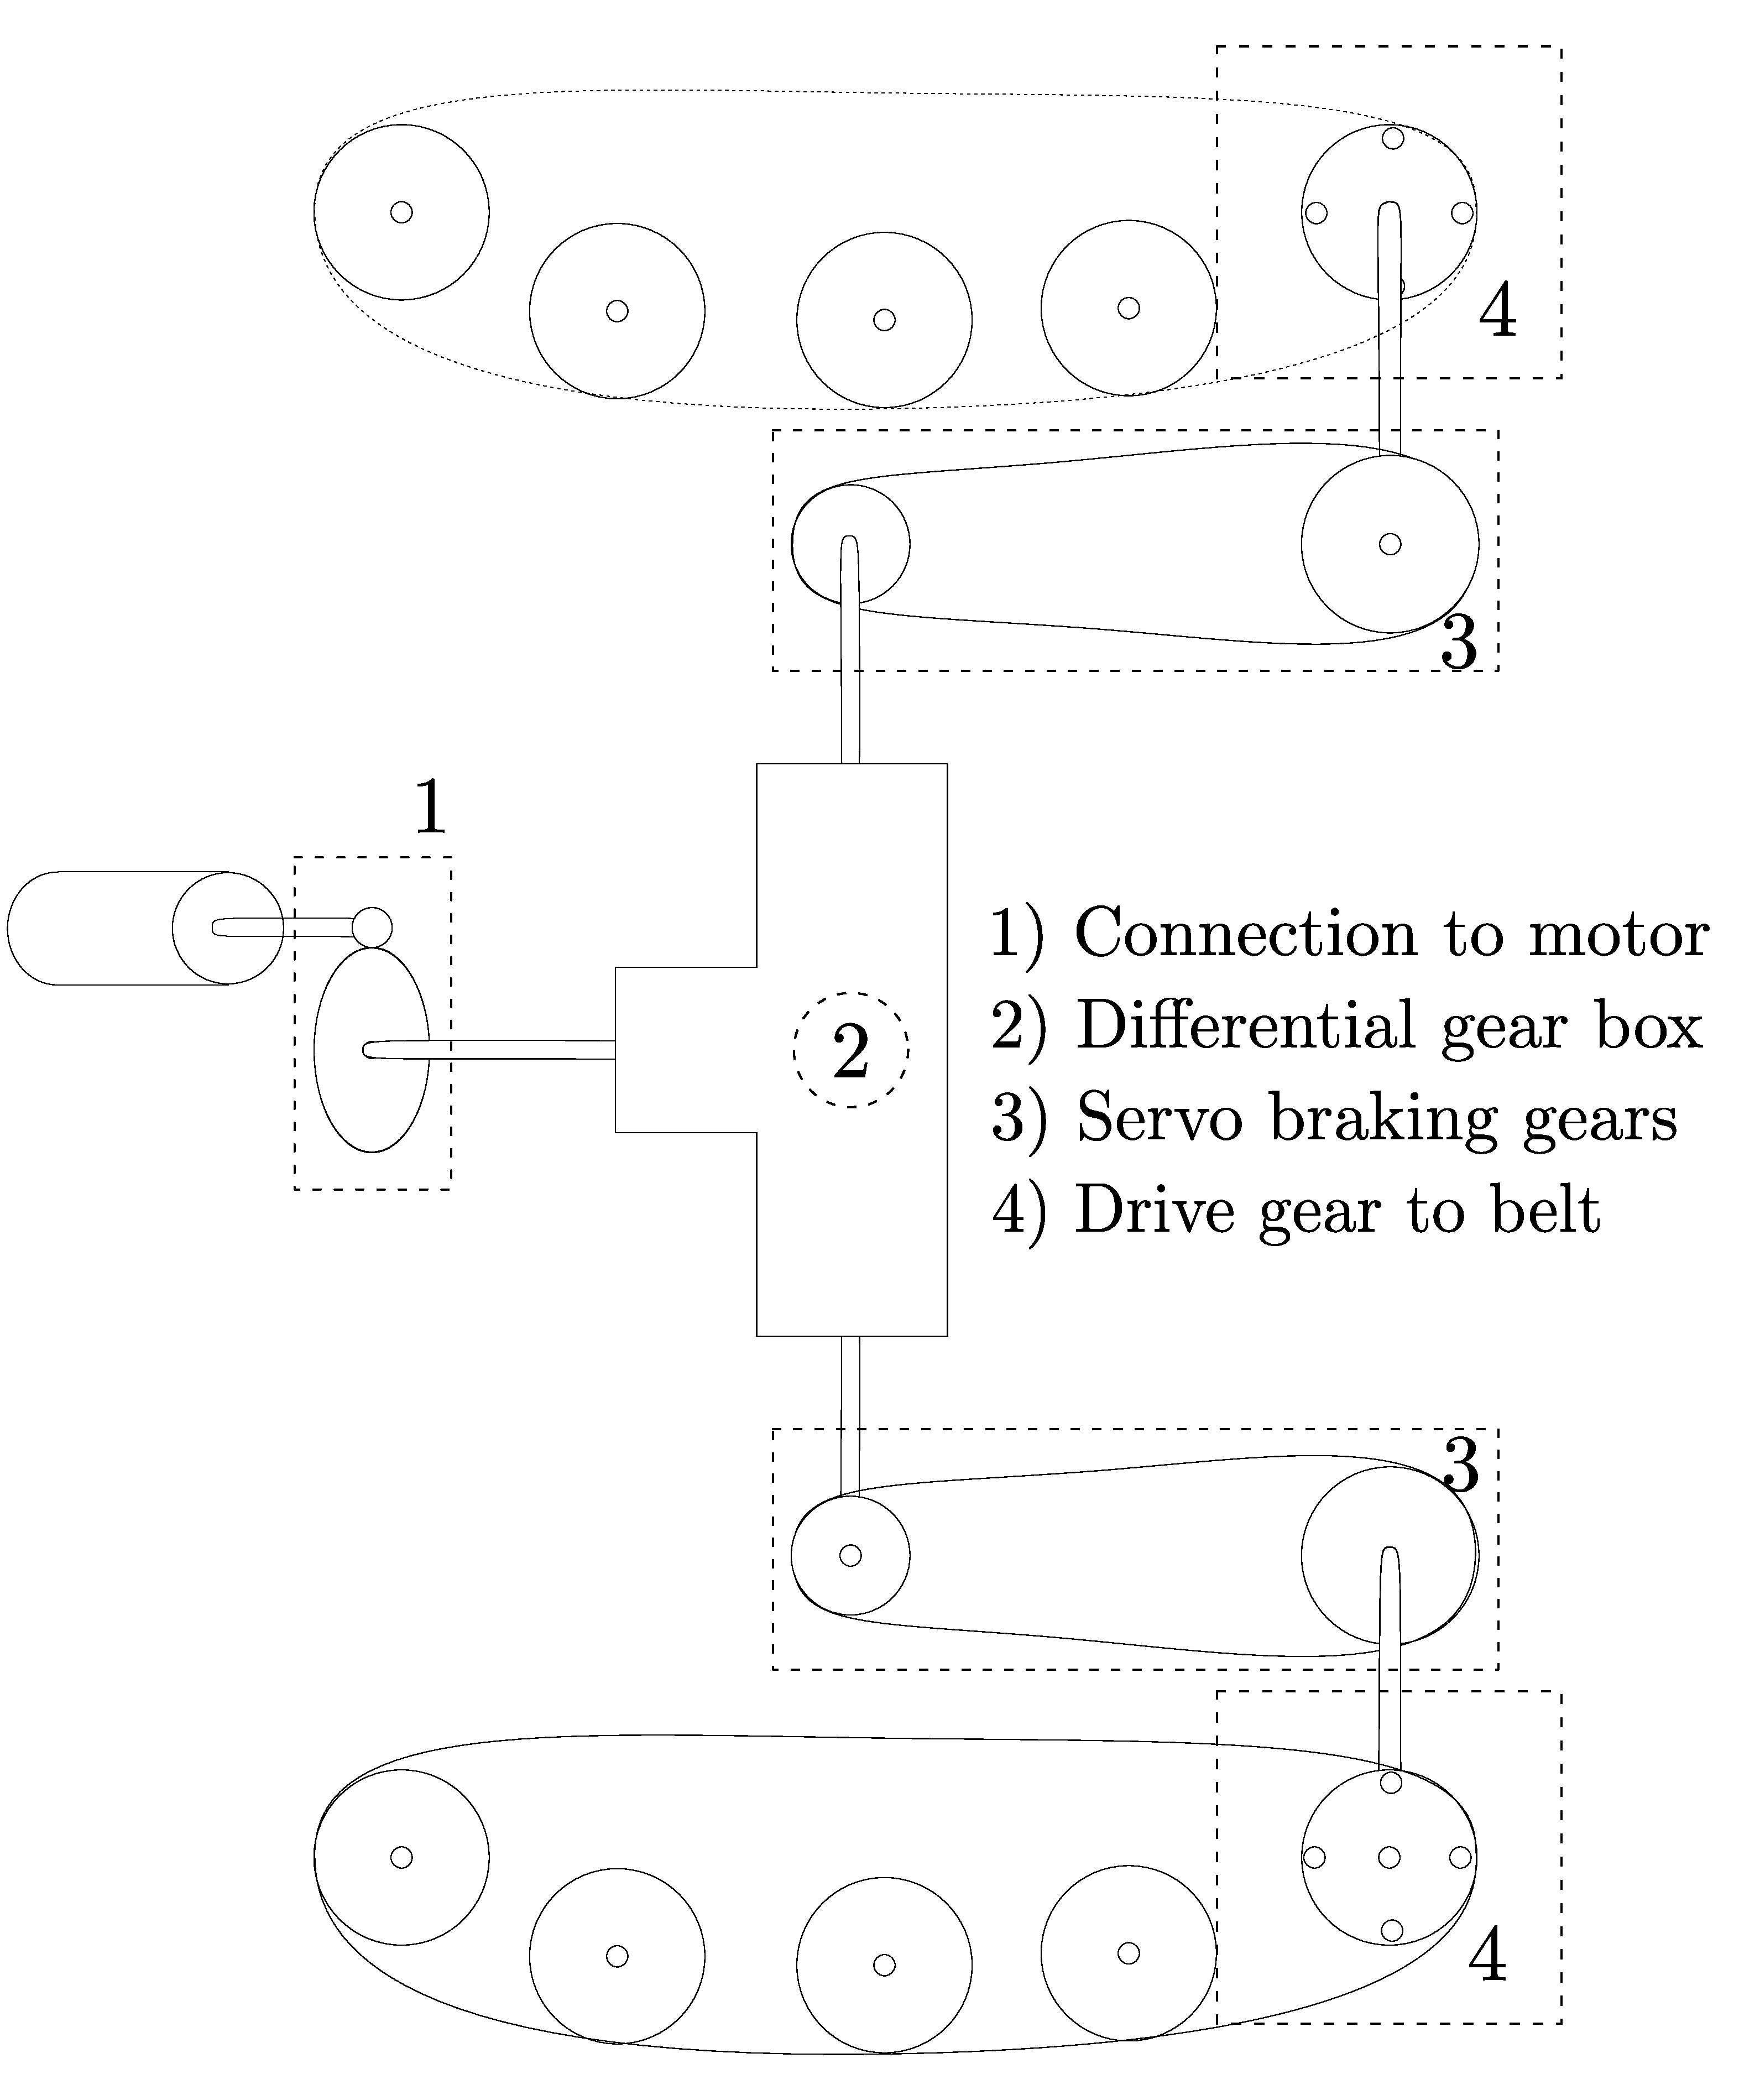
\includegraphics[scale=0.2]{figures/vehicleDescriptionDriveTrain.pdf}
	\caption{Illustration of the drive train of the vehicle.}
	\label{vehicleDescriptionDriveTrain}
\end{figure}

The vehicle is composed of two tracks enveloping 4 wheels, plus a gear connected to the differential gear box. The servomotor in (3) controls the steering of the vehicle by braking one track or another, so that the main motor only control the absolute speed and not the turning. The differential gear, in (2), is powered direcly by the motor.\\
A Hall sensor, in (4), is plugged on each gear wheel to control the speed of each belt.\\
 This section will describe more accurately different part of the vehicle seen in this picture.\\